\documentclass[11pt]{article}

\usepackage{thumbpdf, amssymb, amsmath, amsthm, microtype,
	    graphicx, verbatim, listings, color, fancybox}
\usepackage[pdftex]{hyperref}
%\usepackage[margin=1in]{geometry}
\usepackage{cawsty}
\usepackage{fullpage}
\usepackage{pseudocode}
\usepackage{verbatim}
\usepackage{multicol}

\usepackage{fancybox}
\usepackage{tikz}

\newcommand{\tlg}{\text{lg}}
\newcommand{\tln}{\text{ln}}
\newcommand{\tlog}{\text{log}}

\usepackage{algorithm}
%\usepackage{algorithmic}
\usepackage{amsmath}
\usepackage{amsthm}
\usepackage{algpseudocode}
\usepackage{algorithmicx}% http://ctan.org/pkg/algorithmicx
\usepackage{lipsum}% http://ctan.org/pkg/lipsum
\usepackage{xifthen}% http://ctan.org/pkg/xifthen
\usepackage{needspace}% http://ctan.org/pkg/needspace
\usepackage{hyperref}% http://ctan.org/pkg/hyperref

\usepackage{tikz}
\usetikzlibrary{arrows,%
                shapes,positioning}

\tikzstyle{vertex}=[circle,fill=black!25,minimum size=20pt,inner sep=0pt]
\tikzstyle{selected vertex} = [vertex, fill=red!24]
\tikzstyle{edge} = [draw,thick,-]
\tikzstyle{weight} = [font=\small]
\tikzstyle{selected edge} = [draw,line width=5pt,-,red!50]
\tikzstyle{ignored edge} = [draw,line width=5pt,-,black!20]

\allowdisplaybreaks[1]

% ================ ALGORITHM ENVIRONMENT ================
\newcounter{numberedAlg}% Algorithm counter
\newenvironment{numberedAlg}[1][]%
  {% \begin{numberedAlg}[#1]
    \needspace{2\baselineskip}% At least 2\baselineskip required, otherwise break
    \noindent \rule{\linewidth}{1pt} \endgraf% Top rule
    \refstepcounter{numberedAlg}% For correct reference of algorithm
    \centering \textsc{Algorithm}~\thenumberedAlg%
    \ifthenelse{\isempty{#1}}{}{:\ #1}% Typeset name (if provided)
  }{% \end{numberedAlg}
  \noindent \rule{\linewidth}{1pt}% Bottom rule
  }%

%\setlength{\parindent}{0pt}

\linespread{1.2}

\begin{document}
\cawtitle{4005-800 Algorithms}{Homework 5}

\begin{prob}{1-a}
\end{prob}
\begin{sol}

To find the optimal parenthesization of a matrix chain product whose sequence of dimensions is $<5, 10, 3, 12, 5, 50, 6>$, we simply use the $minMuls$ and $genParens$ functions to find the optimal number of multiplications and then insert the right parentheses, respectively. The steps of the mulMuls algorithm is shown below.

\begin{table*}[htbp]
	\centering
	\begin{tabular}{|l|l|l|l|l|l|}
		 \hline
        0 & - & - & - & - & - \\ 
        - & 0 & - & - & - & - \\ 
        - & - & 0 & - & - & - \\ 
        - & - & - & 0 & - & - \\ 
        - & - & - & - & 0 & - \\ 
        - & - & - & - & - & 0 \\
        \hline
	\end{tabular}
	\hspace{20mm}
	\begin{tabular}{|l|l|l|l|l|l|}
		 \hline
        - & - & - & - & - & - \\ 
        - & - & - & - & - & - \\ 
        - & - & - & - & - & - \\ 
        - & - & - & - & - & - \\ 
        - & - & - & - & - & - \\ 
        - & - & - & - & - & - \\
        \hline
	\end{tabular}
	\caption{$m$ and $c$ tables for $l = 1$ (base case)}
\end{table*}

\begin{table*}[htbp]
	\centering
	\begin{tabular}{|l|l|l|l|l|l|}
		 \hline
        0 & 150 & - & - & - & - \\ 
        - & 0 & 360 & - & - & - \\ 
        - & - & 0 & 180 & - & - \\ 
        - & - & - & 0 & 3000 & -\\ 
        - & - & - & - & 0 & 1500  \\ 
        - & - & - & - & - & 0 \\
        \hline
	\end{tabular}
	\hspace{20mm}
	\begin{tabular}{|l|l|l|l|l|l|}
		 \hline
        - & 1 & - & - & - & - \\ 
        - & - & 2 & - & - & - \\ 
        - & - & - & 3 & - & - \\ 
        - & - & - & - & 4 & - \\ 
        - & - & - & - & - & 5 \\ 
        - & - & - & - & - & - \\
        \hline
	\end{tabular}
	\caption{$m$ and $c$ tables for $l = 2$}
\end{table*}

\begin{table*}[htbp]
	\centering
	\begin{tabular}{|l|l|l|l|l|l|}
		 \hline
        0 & 150 & 330 & - & - & - \\ 
        - & 0 & 360 &330 & - & - \\ 
        - & - & 0 & 180 & 930 & - \\ 
        - & - & - & 0 & 3000 & 1860\\ 
        - & - & - & - & 0 & 1500  \\ 
        - & - & - & - & - & 0 \\
        \hline
	\end{tabular}
	\hspace{20mm}
	\begin{tabular}{|l|l|l|l|l|l|}
		 \hline
        - & 1 & 2 & - & - & - \\ 
        - & - & 2 & 2 & - & - \\ 
        - & - & - & 3 & 4 & - \\ 
        - & - & - & - & 4 & 4 \\ 
        - & - & - & - & - & 5 \\ 
        - & - & - & - & - & - \\
        \hline
	\end{tabular}
	\caption{$m$ and $c$ tables for $l = 3$}
\end{table*}

\begin{table*}[htbp]
	\centering
	\begin{tabular}{|l|l|l|l|l|l|}
		 \hline
        0 & 150 & 330 & 405 & - & - \\ 
        - & 0 & 360 &330 & 2430 & - \\ 
        - & - & 0 & 180 & 930 & 1770 \\ 
        - & - & - & 0 & 3000 & 1860\\ 
        - & - & - & - & 0 & 1500  \\ 
        - & - & - & - & - & 0 \\
        \hline
	\end{tabular}
	\hspace{20mm}
	\begin{tabular}{|l|l|l|l|l|l|}
		 \hline
        - & 1 & 2 & 2 & - & - \\ 
        - & - & 2 & 2 & 2 & - \\ 
        - & - & - & 3 & 4 & 4 \\ 
        - & - & - & - & 4 & 4 \\ 
        - & - & - & - & - & 5 \\ 
        - & - & - & - & - & - \\
        \hline
	\end{tabular}
	\caption{$m$ and $c$ tables for $l = 4$}
\end{table*}

\begin{table*}[htbp]
	\centering
	\begin{tabular}{|l|l|l|l|l|l|}
		 \hline
        0 & 150 & 330 & 405 & 1655 & - \\ 
        - & 0 & 360 &330 & 2430 & 1950 \\ 
        - & - & 0 & 180 & 930 & 1770 \\ 
        - & - & - & 0 & 3000 & 1860\\ 
        - & - & - & - & 0 & 1500  \\ 
        - & - & - & - & - & 0 \\
        \hline
	\end{tabular}
	\hspace{20mm}
	\begin{tabular}{|l|l|l|l|l|l|}
		 \hline
        - & 1 & 2 & 2 & 4 & - \\ 
        - & - & 2 & 2 & 2 & 2 \\ 
        - & - & - & 3 & 4 & 4 \\ 
        - & - & - & - & 4 & 4 \\ 
        - & - & - & - & - & 5 \\ 
        - & - & - & - & - & - \\
        \hline
	\end{tabular}
	\caption{$m$ and $c$ tables for $l = 5$}
\end{table*}

\begin{table*}[htbp]
	\centering
	\begin{tabular}{|l|l|l|l|l|l|}
		 \hline
        0 & 150 & 330 & 405 & 1655 & 2010 \\ 
        - & 0 & 360 &330 & 2430 & 1950 \\ 
        - & - & 0 & 180 & 930 & 1770 \\ 
        - & - & - & 0 & 3000 & 1860\\ 
        - & - & - & - & 0 & 1500  \\ 
        - & - & - & - & - & 0 \\
        \hline
	\end{tabular}
	\hspace{20mm}
	\begin{tabular}{|l|l|l|l|l|l|}
		 \hline
        - & 1 & 2 & 2 & 4 & 2 \\ 
        - & - & 2 & 2 & 2 & 2 \\ 
        - & - & - & 3 & 4 & 4 \\ 
        - & - & - & - & 4 & 4 \\ 
        - & - & - & - & - & 5 \\ 
        - & - & - & - & - & - \\
        \hline
	\end{tabular}
	\caption{$m$ and $c$ tables for $l = 6$}
\end{table*}

Now, using these values, we conclude that the minimum number of multiplications needed to evaluate this sequence of matrices is 2010. Since the sequence $<5, 10, 3, 12, 5, 50, 6>$ corresponds to the matrices $A_1$ (5 x 10), $A_2$ (10 x 3), $A_3$ (3 x 12), $A_4$ (12 x 5), $A_5$ (5 x 50), $A_6$ (50 x 6), respectively, we can now find the optimal parenthesization using the resulting $c$ matrix, which yields the following result: \\ 

$((A_1A_2)(A_3A_4)(A_5A_6))$

\end{sol}

\begin{prob}{1-b}
Show that a fully parenthesization of an $n$-element expression has exactly $n-1$ pairs of parentheses.
\end{prob}
\begin{sol}
We can prove this fact using induction on the number of matrices in a matrix chain. \\
\textbf{Base \#1:} $n = 1$ \\
By definition, an expression is fully parenthesized if it is a single element. Therefore, since $n=1$ corresponds to an expression of a single element (a single matrix), then we know it is fully parenthesized with no parentheses. Thus, we have $(1-1) = 0$ parentheses for a $n = 1$ element expression.\\
\textbf{Base \#2:} $n = 2$ \\
By definition, a $2$-element expression is fully parenthesized if it is the product of the two fully parenthesized elements surrounded by a single pair of parenthesis. Since single elements are fully parenthesized by themselves with no addition parenthesis, we know that an $2$-element expression is fully parenthesized if we write it as the product of the two elements surrounded by parentheses. Thus, with this $2$-element expression, we can make it fully parenthesized with $2-1 = 1$ pair of parentheses. \\
\textbf{Induction:} $n = 2$ \\
Assume that a full parenthesization of a $k$-element expression has exactly $k-1$ pairs of parentheses. Now, let $[A_1, A_2, ..., A_{k}]A_{k+1}$ be a $k+1$-element expression. By the induction hypothesis, we know that $[A_1, A_2, ..., A_{k}]$ is fully parenthesized with $k-1$ parentheses. Now, since $A_{k+1}$ is a single matrix we know that it is also fully parenthesized with $0$ parentheses, so we can make the full expression $[A_1, A_2, ..., A_{k}]A_{k+1}$ by rewriting it as $([A_1, A_2, ..., A_{k}]A_{k+1})$ (since it is the product of two fully parenthesized expressions). Now, since $[A_1, A_2, ..., A_{k}]$ contributed $k-1$ parentheses and we have just added one more pair of parentheses, the total is now $k$, which is equal to exactly $(k+1) - 1$. \\ \\
Thus, we can see that a fully parenthesization of an $n$-element expression has exactly $n-1$ pairs of parentheses. This can also be argued by observing that a pair of parentheses always wraps two operands with a single operator, and since there are $n-1$ operators in an $n$-element expression, there must also be $n-1$ parentheses if it is fully parenthesized.
\end{sol}

\begin{prob}{2-a}
Which is a more efficient way to determine the optimal number of multiplications in a matrix-chain multiplication problem: enumerating all the ways of parenthesizing the product and computing the number of multiplications for each, or running the recursive matrix chain algorithm?
\end{prob}
\begin{sol}
Running the RECURSIVE-MATRIX-CHAIN algorithm is more efficient than exhausting enumeration of the possible parenthesization of the matrix chain. Informally, it is easy to see that the recursion tree for the RECURSIVE-MATRIX-CHAIN algorithm does not contain all possible enumerations for the different parenthesization schemes for a given matrix chain. For each subproblem from index $i$ to $j$ that is solved by the RECURSIVE-MATRIX-CHAIN algorithm, we can see that the optimal midpoint in the chain from matrix $i$ to matrix $j$ is found recursively using two subproblem invocations of RECURSIVE-MATRIX-CHAIN on the left and right half of this midpoint, and then those results are simply combined to obtain the optimal result for matrices from index $i$ to $j$. However, using the enumeration approach, we would calculate all  parenthesization possibilies for all possible left and right halves of the matrix chain from $i$ to $j$, and then we would have to compute the result of all possible combinations of these left and right half possibilities to find the optimal value for the chain from $i$ to $j$. Basically, the RECURSIVE-MATRIX-CHAIN  algorithm only does one combination step after the left and right subproblems have been solved to find the optimal value, whereas the enumeration approach performs many combinations for left and right half partitions until it finds the optimal value. Thus, by this simple argument, we can see that the RECURSIVE-MATRIX-CHAIN algorithm is by far more efficient than the enumeration approach.

Formally, we know (by section 15.2 in the textbook) that the enumeration approach runs in $\Omega(\frac{4^n}{n^{3/2}})$ (similar to the \emph{Catalan numbers}. To show that the RECURSIVE-MATRIX-CHAIN algorithm is computationally more efficient, we must establish an upper bound on its time complexity that is less than the enumeration approach. With this as motivation, we first identify a recurrence $T(n)$ for the time of the RECURSIVE-MATRIX-CHAIN algorithm as follows:

\[
T(n) = \left\{ 
  \begin{array}{l l}
    1, & \quad \text{if $n = 1$}, \\
    1 + \sum_{k=1}^{n-1}(T(k) + T(n-k) + 1), & \quad \text{if $n > 1$}. \\
  \end{array} \right.
\]

This is from the observation that the comparison and multiplication operations in the RECURSIVE-MATRIX-CHAIN algorithm take constant time $(O(1))$, and at each step in the partition loop we are making two recursive calls, where the size of the index range for each recursive call adds up to $n$. We can make a further observation that, if the inner sum was split up, the $T(k)$ and $T(n-k)$ terms could be rewritten as $T(k)$ and $T(k)$, which implies that we can rewrite $T(n)$ as follows:

\[
T(n) = \left\{ 
  \begin{array}{l l}
    1, & \quad \text{if $n = 1$}, \\
    1 + \sum_{k=1}^{n-1}(2T(k) + 1), & \quad \text{if $n > 1$}. \\
  \end{array} \right.
\]

Evaluating this recurrence by treating it as a recurrence with full history, and assuming that $T(2) = 3$, we obtain the following:
\begin{eqnarray*}
T(n) - T(n - 1) & = & (n - 1) - (n - 2) + 2T(n-1) \\
\end{eqnarray*}
Simplifying and evaluation this expression yields the following:
\begin{eqnarray*}
T(n) & = & 1 + 3T(n-1) \\
& = & 1 + 3(1 + 3T(n-2)) \\
& = & 1 + 3(1 + 3(1 + 3T(n-3))) \\
& = & ... \\
& = & \sum_{k=0}^{n-3}3^k + 3^{n-2}T(2) \\
& = & \frac{3^{n-2} - 1}{2} + 3^{n-2}(3) \\
& = & \frac{1}{2}(3^{n-2} + 2(3^{n-1}) - 1) \\
& < & \frac{1}{2}(3^{n-2} + n(3^{n-1}) - 1) \\
& = & O(n3^{n-1})
\end{eqnarray*}
Thus, since $T(n) = O(n3^{n-1})$ and the enumeration approach has a time complexity of $\Omega(\frac{4^n}{n^{3/2}})$, we can conclude that the RECURSIVE-MATRIX-CHAIN does indeed run more efficiently. 
\end{sol}

\begin{prob}{2-b}
Draw the recursion tree for the MERGE-SORT procedure from Section 2.3.1 on an array of 16 elements. Explain why memoization fails to speed up a good divide-and-conquer algorithm such as MERGE-SORT.
\end{prob}
\begin{sol} \\

\ovalbox{
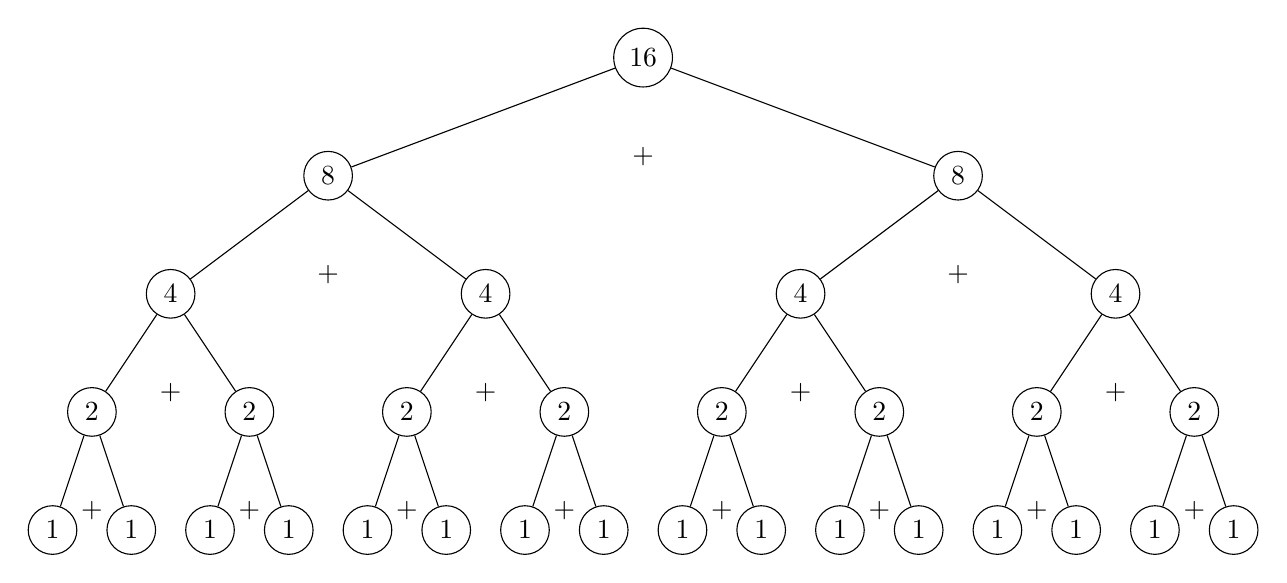
\begin{tikzpicture}[
auto,
level 1/.style={sibling distance=80mm},
level 2/.style={sibling distance=40mm},
level 3/.style={sibling distance=20mm},
level 4/.style={sibling distance=10mm}]
\node [circle,draw] (z){$16$}
  child {
	node [circle,draw] (a) {$8$}
    	child {
		node [circle,draw] (b) {$4$}
      		child {
			node [circle,draw] (c) {$2$}
        		child {
				node [circle,draw] (d) {$1$}
			}
        		child {
				node [circle,draw] (e) {$1$}
			}
      		} 
     		child {
			node [circle,draw] (f) {$2$}
        		child {
				node [circle,draw] (g) {$1$}
			}
        		child {
				node [circle,draw] (h) {$1$}
			}
      		} 
    	}
   	child {
		node [circle,draw] (b1) {$4$}
      		child {
			node [circle,draw] (c1) {$2$}
        		child {
				node [circle,draw] (d1) {$1$}
			}
        		child {
				node [circle,draw] (e1) {$1$}
			}
      		} 
      		child {
			node [circle,draw] (f1) {$2$}
        		child {
				node [circle,draw] (g1) {$1$}
			}
        		child {
				node [circle,draw] (h1) {$1$}
			}
      		} 
    	}
  }
  child {
	node [circle,draw] (ar) {$8$}
    	child {
		node [circle,draw] (br) {$4$}
  	  	child {
			node [circle,draw] (cr) {$2$}
        		child {
				node [circle,draw] (dr) {$1$}
			}
        		child {
				node [circle,draw] (er) {$1$}
			}
      		} 
      		child {
			node [circle,draw] (fr) {$2$}
        		child {
				node [circle,draw] (gr) {$1$}
			}
        		child {
				node [circle,draw] (hr) {$1$}
			}
      		}	 
    	}
    	child {
		node [circle,draw] (br1) {$4$}
      		child {
			node [circle,draw] (cr1) {$2$}
        		child {
				node [circle,draw] (dr1) {$1$}
			}
        		child {
				node [circle,draw] (er1) {$1$}
			}
      		} 
      		child {
			node [circle,draw] (fr1) {$2$}
        		child {
				node [circle,draw] (gr1) {$1$}
			}
        		child {
				node [circle,draw] (hr1) {$1$}
			}
      		} 
    	}
};
\path (a) -- (ar) node [midway] {+};
\path (b) -- (b1) node [midway] {+};
\path (c) -- (f) node [midway] {+};
\path (d) -- (e) node [midway] {+};
\path (g) -- (h) node [midway] {+};
\path (c1) -- (f1) node [midway] {+};
\path (d1) -- (e1) node [midway] {+};
\path (g1) -- (h1) node [midway] {+};
\path (br) -- (br1) node [midway] {+};
\path (cr) -- (fr) node [midway] {+};
\path (dr) -- (er) node [midway] {+};
\path (gr) -- (hr) node [midway] {+};
\path (cr1) -- (fr1) node [midway] {+};
\path (dr1) -- (er1) node [midway] {+};
\path (gr1) -- (hr1) node [midway] {+};
\end{tikzpicture}}\\

This same recursion tree can be shown using arrays instead, as depicted below.

\begin{center}
	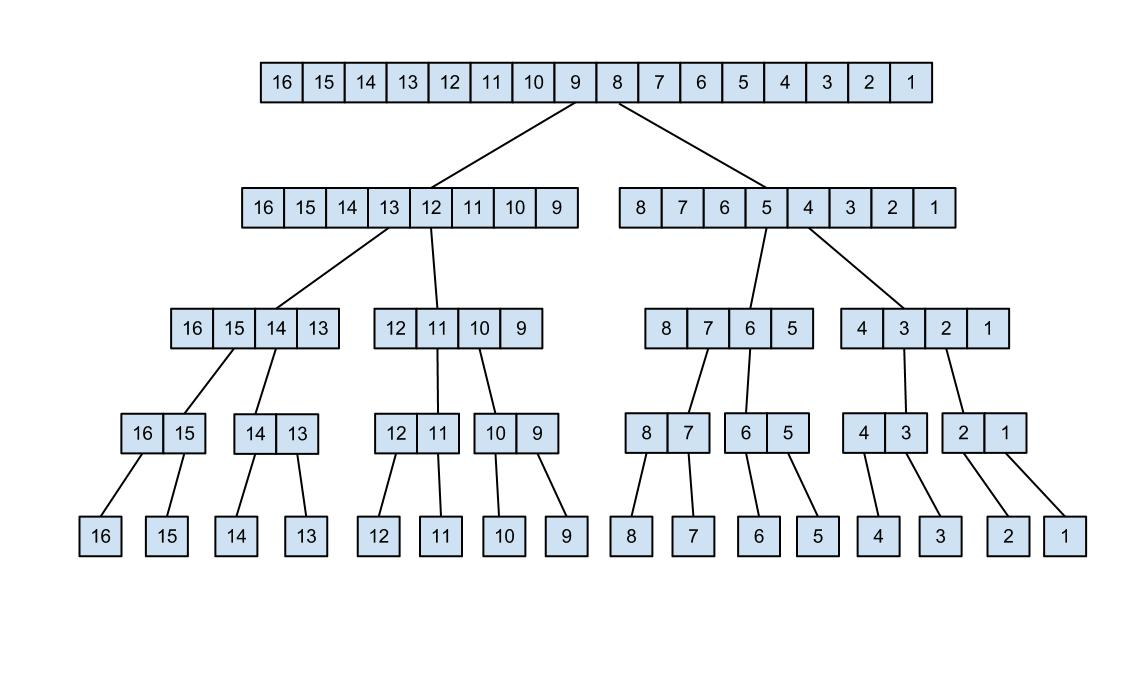
\includegraphics[width=150mm]{msort16.jpg}
\end{center}

One can see that there is no overlap in the sorting subproblems for this specific input array to mergesort, meaning that no there is not an instance where two identitical sub-arrays are passed into mergesort. 

Memoization fails to speed up a good divide-and-conquer algorithm such as MERGE-SORT because there are no overlapping subproblems. Memoization is most beneficial when the results of subproblems can be saved in a table using the top-down recursion approach and then recalled when they are encountered at later recursive calls. As shown by the merge-sort recursion tree, there are no overlapping subproblems, so we will never attempt to sort the same subsequences more than once. Thus, we would never make use of the sorted subsequences that have been stored, and will consequently not see any speedup. Other good divide-and-conquer algorithms yield the same results, because the subproblems that are solved recursively are chosen such that they are independent and do not overlap. 
\end{sol}

\begin{prob}{2-c}
Consider a variant of the matrix-chain multiplication problem in which the goal is to parenthesize the sequence of matrices so as to maximize, rahter than minimize, the number of scalar multiplications. Does this problem exhibit optimal substructure?
\end{prob}
\begin{sol}
Yes, this problem does exhibit optimal substructure. As with the minimization version of the problem, the optimal solution entails making a choice among two subproblems (the two partitions of the matrix-chain) as to which should be used to yield the maximum number of scalar multiplications. In addition, because matrix multiplication is not commutative, we are forced to maintain the same order of the matrix chain, and thus both partitions that represent the two subproblems involved in the optimal calculation are independent. In other words, the optimal solution to the left partition of the matrix-chain (the optimal number of scalar multiplications) does not affect the optimal solution to the right partition of the matrix-chain. Therefore, since the optimal value is obtained by making a choice among two subproblems that are independent, we can conclude that this problem variant yields optimal substructure.
\end{sol}

\begin{prob}{3}
\end{prob}
\begin{sol}
TODO - describe the algorithm here and the approach taken - insert code - show correctness
\end{sol}

\end{document}
